
%*********************第三章******************
\chapter{心脏组织模拟在天河2异构系统上的并行优化}
\label{icpads}

\section{引言}
在\ref{ICA3PP}中,已经介绍了心脏组织模拟在研究心律失常等各种心脏疾病具有重要的作用,心脏组织模拟的模型越详细,对计算的需求越大,在\ref{ICA3PP}中也已经介绍了本课题在多核CPU的集群系统上做的一些工作,采用了MPI+OpenMP的并行编程方法,对一定规模的心脏组织进行了模拟。但如果想对更大规模的心脏组织模拟则需要计算能力更强的处理器或者加速器构成的超大规模集群系统。文献中\upcite{GPUcell}采用了GPU在细胞层级对模拟进行加速,利用加速器对模拟进行加速不失为一种好的选择。

基于现有的计算资源,本课题将心脏组织模拟移植到超级异构集群系统即天河2号超级计算机\upcite{tianhe}上。天河2号超级计算机系统在TOP500排名中位居第二,它的每个计算节点都是由Intel CPU与Intel PHI协处理器构成的异构系统。

众核加速器的每个芯片集成了大量的简单小核,非常适合作为高性能计算系统的核心计算部件。Intel的Xeon Phi协处理器和GPU是两种典型的众核加速器。本课题将面向天河2号超级计算机系统实现心脏组织的3D模拟,天河2号超级计算机系统采用多核CPU作为控制核心以及Intel Xeon Phi协处理器作为加速部件。天河2号系统的峰值性能可以达到54.9PFlops,实测性能可以达到33.86PFlops。

天河2号系统具有很强的计算能力,但天河2号作为复杂的异构系统,这给天河2号上的并行编程带来了诸多挑战。因此,对于一个应用能否在天河2号上取得很好的性能,取决于并行实现。对于天河2号系统来说,除了需要高效地充分利用其大量的硬件线程,单个物理线程上的SIMD向量化也需要尽可能地得到发挥。物理线程的并行可以通过OpenMP编程实现,或者通过一个MPI进程内创建多个OpenMP线程控制多个物理线程,SIMD向量化理论上能够将双精度的浮点性能提升8倍,SIMD向量化可以在代码中添加编译指导语句,借助编译器对代码自动向量化,或者采用AVX-512向量指令\upcite{XEONPHI}手动对代码进行向量化。编译器自动向量化的方法只针对代码中比较规则的计算,而对于不规则的代码则需要通过手动向量化实现SIMD。

对于由CPU和Xeon Phi构成的异构系统来说,多核CPU的性能同样不容忽略,目前每个计算节点内CPU核的个数一般在8到18之间,然而每个CPU核使用更高的时钟频率,功能也更加强大,更加灵活,适合做一些控制的任务。对于一些特殊的计算,比如很难实现SIMD或者是存储带宽受限,则多核CPU上的实现性能可以达到协处理器上的实现性能。因此异构节点上CPU核与Xeon Phi协处理器应该协同起来,充分发挥异构系统的性能。然而,从编程的角度来说,异构计算可能带来新的问题,比如,对于SIMD向量化,CPU采用不同的AVX指令集,因为CPU的SIMD指令是针对256位的向量计算。异构计算还可能需要解决优化CPU和Xeon Phi间的数据传输问题以及CPU和Xeon Phi间的负载均衡问题等。

本课题的目标是将心脏组织的模拟移植到天河2号的超级异构计算机系统中,为了有效地使用天河2号的硬件资源,需要将模拟的计算过程进行多层次的并行开发,包括计算节点间的并行、节点内CPU和Phi设备间的并行、Phi设备上众核间的并行以及Phi设备的每个计算核心内SIMD的并行。这无疑会给编程带来巨大的挑战,这正是本课题需要解决的问题。

本章内容安排如下,首先将介绍天河2号超级计算机系统的硬件结构;然后将介绍心脏组织模拟在天河2号系统上的高性能并行实现与优化,主要利用硬件结构的特点,将心脏组织模拟的并行映射到具体的硬件中执行,并对其中的关键计算部分进行优化;最后是对试验结果评测,主要测试了心脏组织模拟在天河2号上单节点内的Phi设备上的性能、单节点的性能以及多节点的性能。试验结果表明,本课题针对天河2号异构集群系统开发出了一个高效的心脏组织模拟器。

\section{目标硬件体系结构}

天河2号超级计算系统包含16000个计算节点,每个计算节点有3个Intel Xeon Phi协处理器和2个Intel Xeon E5-2692v2 Ivy Bridge CPU处理器。因此,天河2号系统共有48000个Xeon Phi以及3200个Intel Xeon CPU。Xeon Phi的模型为31S1P(即Knigths Corner体系结构),每个Xeon Phi有57个核心,频率为1.1GHz,每个CPU有12和核心,频率为2.2GHz。

Intel Xeon Phi协处理器是一个基于众核设计的硬件加速器,与传统的多核CPU不同的是,Phi协处理器是由大量的性能相对较弱的小核构成的,这些小核以环形的结构相连,每个小核支持512位宽的向量处理,具有64KB大小的L1 cache以及512KB大小的L2 cache,所有小核的cache支持一致性协议。Xeon Phi的这种设计使得它不适合处理串行程序,但非常适合处理并行程度高的程序。对于Xeon CPU来说,CPU中的每个小核具有64KB大小的L1 cache,256KB大小的L2 cache,并且Xeon CPU具有被12个小核共享的30MB大小的L3 cache。

Xeon Phi的理论峰值双精度性能可以根据参数理论上计算出来,它的向量位宽为512位,所以每次可以处理8个双进度浮点运算或者16个单精度浮点运算,根据前面介绍的频率和小核的个数,可以计算出一个Xeon Phi的单精度浮点峰值性能可以达到$1001$ GFlop/s。然而,在实际中,一般不能取得这么高的性能,CPU的计算性能也不容忽略,峰值性能可以达到$211$ GFlop/s,实际中应该充分发挥Xeon CPU和Xeon Phi两种计算资源的性能。

对于节点间的通信问题,天河2号系统采用了自己定制的名为TH Express-2的互联系统,这是一个胖树的拓扑结构。理论上说,Xeon Phi上是支持MPI通信的,单节点内Xeon Phi间采用MPI通信对性能不会有太大损失,但对于处于不同节点的Xeon Phi间的通信,采用MPI通信并不是很高效的方法。因此,本课题采用的策略是一个节点由一个MPI进程控制,然后在MPI进程内为每一个Xeon Phi创建一个线程,每个线程负责管理一个Xeon Phi,Xeon CPU和Xeon Phi间的通信采用Intel的SCIF/COI接口\upcite{SCIFCOI}进行通信。由于SCIF/COI接口较底层,编程会相对较复杂,但会取得很好的性能。

Xeon Phi的57个小核中,有一个小核是保留给操作系统使用的,因此,真正能用于计算的小核个数只有56个。每个小核能同时运行4个物理线程,但对于给定的一个线程,它不会在连续的两个时钟周期都运行,意味一个Xeon Phi内只有有效的112个线程能以$1.1$ GHz的时钟周期运行。当运行224个线程时,每个线程是以系统的时钟周期的一半运行的。Xeon Phi协处理器的DDR5设备存储大小为8GB,小核访问设备全局存储的峰值带宽\upcite{xeon_phi_peak}为$320$ GB/s。然而,即使在理想情况下,对于很多应用来说,峰值带宽的一半还是可以达到的\upcite{testdrivingPhi}。


\section{心脏组织模拟的高性能并行实现与优化}

本节主要介绍了心脏组织模拟在天河2号超级计算系统上的映射。根据心脏组织模拟应用本身的并行特点,开发出各种并行性,并且将将这种并行映射到天河2号的硬件体系结构中。

\subsection{心脏组织模拟的tissue-级并行}
\label{tissueParallel}
心脏组织模拟的全部计算任务具有多个层次的并行性,结合目标体系结构的特点,本课题对心脏组织模拟的计算任务进行分解,分解成多个层次。在最顶层分解中,心脏组织细胞以3D网格的方式结合在一起。每一个计算节点被分配到一定数量的细胞进行处理,这些细胞构成一个子域,子域的形状也是一个立方体。处于子域边界的细胞,它们的电压值在进行扩撒计算前需要与相邻的子域边界的细胞的电压值交换。细胞的电压值交换是通过CPU间的MPI通信实现的,采用了标准的halo交换方法。

对于每个子域在节点内的CPU和Phis间的细胞划分,本课题没有对立方体构成的子域进行规则的划分,因为这会导致CPU与Phis间负载的不均衡,而是根据CPU和Phi的计算能力分配相应比例的细胞给CPU和Phi这两种计算设备。这种策略需要对CPU和Phis处理的所有的细胞的电压值进行交换,CPU和Phi间的通信采用Intel的SCIF/COI通信接口实现。虽然这种方法会增加节点内CPU和Phi间的通信,但付出的代价会比因为负载不均问题产生的额外开销小。图\ref{nodeload}是节点内对子域构成的立方体细胞划分的示意图,不同颜色的部分代表分配给不同的计算设备。

 \begin{figure}[bth]
\center
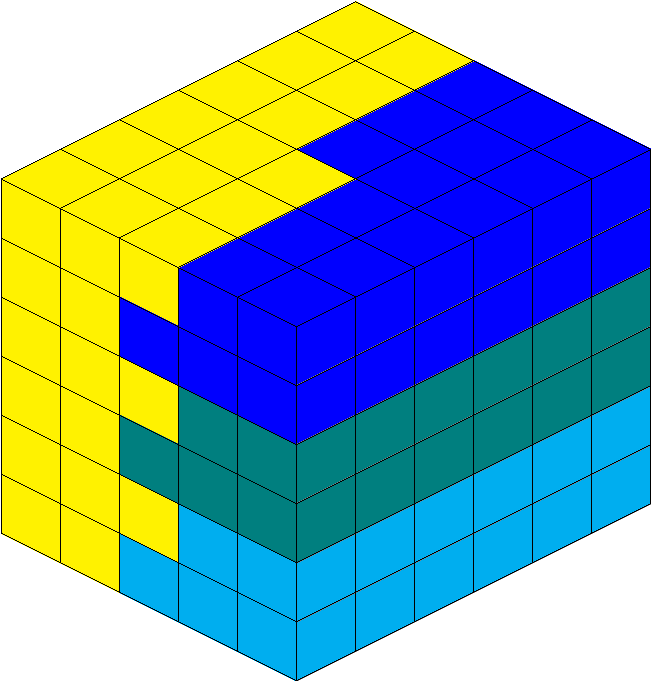
\includegraphics[scale=0.5]{figs/cube}
\caption{Example of the intra-node decomposition of a subdomain. Cells allocated to the Phis are shown in \textcolor{blue}{blue}, \color{teal}{teal}, \textcolor{black}{and} \textcolor{cyan}{cyan}, \textcolor{black}{while the CPU cells are shown in} \textcolor{yellow}{yellow}.}
\label{nodeload}
\end{figure}

另外,因为每个细胞内含有大量的dyad单元,在代码实现中,每个细胞大约需消耗3MB的存储,受限于Phi设备的8GB的DDR存储以及Phi设备同时最多运行224个线程,导致每个Phi设备最多只能处理2500个细胞,这意味着每个线程每个时间步也只能计算少量的细胞,这使得整体性能对负载均衡非常敏感。因此,为每个Phi设备分配的细胞数最好是224的整数倍,这有利于设备内线程的负载均衡。

在前期的试验结果发现天河2号的每个计算节点内,2个CPU的性能与单个Phi实测的性能比约为$1.5 : 1$。根据上述限制,本课题为每一个节点分配的细胞规模为$20\times20\times20$,$8\times224=1792$ 个细胞分配给一个Phi设备,剩下$8000-3\times1792=2624$个细胞分配给主机上的2个CPU进行计算。CPU处理的细胞数大约占单个节点内任务的$32.8\%$,同样的比例同样适用其它大小规模的子域。然而,实际测试中,针对不同的子域,CPU和Phi设备的性能还是存在细微的差异,因此,要做到完美的负载均衡是不太可能的。

 
\subsection{心脏组织模拟的cell-级并行}
正如\ref{tissueParallel}中提到的负载均衡问题,本课题采用了一种直接而静态的分配策略,即事先将细胞固定指定到相应的计算设备中执行,并且细胞内的所有计算自始自终都在同一个小核中完成的。与静态分配策略相对应的是动态分配策略,每个细胞内特别是所有dyad内的计算由所有的计算核心共同完成,这种方法可以更好地缓解负载均衡的问题。但由于部分计算必须串行执行,在计算过程中会导致重要的延迟。

因此,在每个小核中,本课题采用SIMD向量单元并行处理4个(CPU)或者8个(Phi)细胞内钙离子释放单元的计算。向量化对模拟实现的性能具有重要的影响作用,由于模拟过程的复杂性,本课题采用混合并行化的方法,包括由Intel icc编译器完成的自动编译方法和利用Intel 向量化指令实现的手动向量化方法。为了实现混合并行化的方法,对源代码实现中的dyad循环分割成多个小的循环将变得很有必要。因为dyad内部的计算中,既有很规则的计算部分,记为\textit{arithmetic}段,也有部分含有大量控制语句的代码,记为\textit{conditional}段。对于循环中的规则计算,编译器可以很容易对其向量化,然而,对于大量控制语句的代码,编译器很难实现自动化。因此,在对dyad循环内部的计算分割成多个循环之后,规则的循环可以通过编译器自动向量化,而非规则的计算通过手动向量化,这可以大大简化并行优化的工作。

上述说的\textit{arithmetic}段的计算包括决定L-型通道或者RyR状态转变概率、计算钙离子浓度以及计算dyad间的扩散。它们的计算都比较规则,只需要在循环外加上适当的编译指导语句,编译器就能对这些代码自动实现向量化。虽然,dyad间的扩散部分是存储受限并且只包含少量的计算,向量化同样适用,只是提升的性能不是那么显著。\textit{conditional}段包含的从二项分布中采样决定RyR中发生状态转变的数目,由于这部分计算需要{\it while}循环或者等价功能的代码,编译器对这部分代码不能自动实现向量化。

将大循环分割成多个小循环技术的弱点在于降低了数据局域性,对于大循环来说,只需要存储最终的计算结果,因为循环能保证一次性将结果计算出来,而当大循环分割成很多小循环之后,最终的计算结果依赖中间各个阶段的计算结果,需要额外的数组存储这些中间结果,临时中间结果在前半部分被计算出来写到全局存储中,在后半部分计算又从全局存储中读出,这增加了存储带宽的压力。为了避免反复访存,可以考虑将部分循环合并,这就需要手动实现合并之后循环内所有的计算代码。

\subsection{二项分布采样的向量化实现}
对于\textit{conditional}中的代码,可以采用AVX-512指令进行手动向量化,向量化条件语句代码的关键就在于强大的\texttt{mask}指令。\texttt{mask}指令允许SIMD向量单元在执行向量指令时,只对部分元素按照指令执行,针对的元素取决于一个位掩码。AVX-512指令只能在Phi设备上执行,在Sandy Bridge结构的CPU上缺少相应的AVX指令,因此,在针对CPU的代码中,二项分布采样的实现中未进行手动向量化。

AVX-512向量化的实现可以参考图\ref{Vecbinom}。该向量化代码是通过同时计算8个dyad的累积概率分布函数实现采样的,以{\tt N, P}和{\tt RANDVAL}两个向量作为输入,它们包含处在某状态的通道数、转化概率以及针每个dyad采样的一个随机数。采样的结果{\it K},即改变状态的RyR的个数是通过将{\tt RANDVAL}减去二项分布采样的累积概率,直至结果变为负值,需要经过的循环次数$i$而得到。当{\tt RANDVAL}中的某个分量达到负值时,对应的{\tt MASK}将被设置成$0$,而{\tt K}中对应的分量将保持不变。RyR和L型通道转变的处理采用了相同的二项分布采样的方法,为了可读性的方便,这里只介绍了RyR的采样过程。

\begin{figure}[hbt]
\small\begin{verbatim}
function VectorizedBinomial
Input: Vectors N, P, RANDVAL
Output: Vector K
   Initialize K = 0
   Initialize 1P = Vector_subtract(1,P);
   Initialize PKNK = Vector_power(1P,N);
   Initialize P1P = Vector_divide(P,1P);
   for (int i = 0; i < max(N); i++) {	
       BC = Vector_gather(BC_table,N,K);
       SUB = Vector_multiply(BC,PKNK);
       RANDVAL = Vector_subtract(RANDVAL,SUB);
       PKNK = Vector_multiply(P1P,PKNK);
       MASK = Vector_mask_compare(RANDVAL > 0);
       K = Vector_mask_add(K,1,MASK); }
\end{verbatim}
\caption{The vectorized version of the binomial sampling computation. It can be derived from a scalar implementation via the use of MASK to increase the output value for some vector elements, instead of using a \texttt{while} loop. Vector intrinsics are renamed for clarity.}
\label{Vecbinom}
\end{figure}

为了节省时间,向量\texttt{PKNK}和向量\texttt{P1P}在初始化会预先被计算出来。由于向量{\tt N}中的每个元素最大值不会超过$100$,二项分布系数的值可以在真正模拟之前预先计算出来并存储在{\tt BC\_table}。这种方法对于CPU这种只适合标量处理的处理器是有利的,但对于每个小核访存带宽受限,计算能力充足的Phi可以消除这项技术的优势。

向量化实现的方法中,最主要的问题就是计算一直持续到最后一次采样结束。这意味着向量化取得的加速效果取决于处在同一个向量中的8个dyad的采样结果差异,如果所有采样结果相差不大,则可以获得近8倍的加速效果,但实际中,这种情况很少出现。另外,测试掩码向量\texttt{MASK}的值是否为0,即所有的采样已经结束,这种条件检验尤其在Phi设备上代价是比较大的。为此,采用了一种折中的方案,即每隔8次循环进行一次条件判断,来决定是否完成采样过程。

这意味着向量{\tt K}中的最大元素越小,采样时间就越短,这种情况也是经常发生的,因为大都RyR状态间的转化概率是很小的,因此,采样结果一般都是比较小的。另外,向量{\tt N}中的某个元素为0,则向量{\tt K}中对应的元素也一般为0,如果是这种情形,则可以不需要计算就得出结果,随机数向量{\tt RANDVAL}可以在后面的采样使用,这可以节约随机数使用的数目。并且注意到,在图\ref{ryrstates}中的状态转化中,从O1状态到C1状态以及从C3状态到C2状态间的转化概率是常数,这意味着累积分布函数是可以预先计算出来的,这可以大大降低采样过程的计算量。

二项分布的采样过程确实不是特别适合向量化处理,采用大量的柏努利试验方法决定RyR通道处于打开状态的方法更有利于向量化的实现,这是由Phi上的\texttt{compare}指令的特点决定的。然而,这种直接的方法需要消耗大量的随机数,随机数生成在Phi设备上并不是特别的高效。因此,本课题并未采用柏努利试验的方法。

\subsection{心脏组织模拟中随机数生成}
为了产生二项分布采样所需的随机数,本课题使用了Intel MKL库中提供的函数\texttt{vdRngUniform},并在每一次时间步迭代之前调用该函数。随机数产生过程在Phi设备上的性能相对CPU上的性能差很多,单核上的性能几乎相差$40$倍。另外,与CPU不同的是,在Phi设备上随机数生成在多核上的扩展性也非常差,这使得随机数生成成为Phi设备上计算的瓶颈之一。

由于\texttt{vdRngUniform}是预先定义好的库函数,本课题并不能对其实现做进一步的优化。然而,正如上面所提到的,可以在使用随机数的时候做些优化,比如,对于通道数为0的各个初始状态转变的计算是可以跳过的,因此,就不需要消耗随机数了,减少了总的随机数的产生,从而减少了随机数产生的时间。为了实现这个方法,使用一个变量记录每次时间步内所使用的随机数的数目,使用了多少随机数,就在下一个时间步中产生多少随机数覆盖掉当前时间步中使用过的随机数,当前时间步未被使用的随机数将在下一个时间步中继续使用。对于每个dyad来说,RyR通道各个状态的数目计算最多需要消耗8个随机数,L型通道状态的计算最多消耗2个随机数,因此每个dyad最多需要消耗10个随机数,采用上述减少随机数的方法之后,平均能减少一半的随机数的使用,意味着随机数产生的时间可以降低一半。

\subsection{代码优化}
尽管x86 CPU和Xeon Phi在体系结构上具有很强的相似性,但在这两种设备上移植程序而都保持很高的性能并不是件简单的任务。在Xeon Phi设备上较低的串行程序性能,较长的向量单元以及很高的计算性能这些特点,与存储带宽上的性能的对比,使得在这种设备上编程时需要重点解决一些挑战。

Xeon Phi加速器计算性能的发挥非常依赖于512位向量单元得到充分利用,完全的向量化实现能使Xeon Phi的双精度性能直接提升8倍,单精度性能提升16倍。对Xeon CPU来说则是,向量化能使双精度性能提升4倍,单精度性能提升8倍。在大部分情况下,可以在代码中插入编译指导语句使得编译器对相应代码实现自动向量化,而对于复杂的代码,则需考虑通过程序员采用向量化的指令手动向量化实现。

对于Xeon CPU来说,AVX向量化不能对所有的双精度的计算类型都提高4倍,因为只有两个双精度除法的硬件单元可以同时执行,正如文献\upcite{notallflopsequal}中所讨论的。这是因为在CPU处理器中,除法几乎比乘法慢20倍,向量化的加速比最后就取决于在除法运算中获得的加速比了。而Xeon Phi中的每个小核能并行处理8个双精度除法运算,不过除法的开销也同样代价较大,因此无论是针对Xeon CPU还是Xeon Phi设备,都应该尽量减少对除法的使用,比如可以用乘法代替除法,不过,这都需要手动实现,因为编译器无法自动实现乘法操作对除法的替换工作。

对于细胞内的dyad间的扩散计算,编译器也可以实现该部分计算的自动向量化,并且能够取得一定性能的提升。一种有效的模板计算的实现是避免使用条件分支语句,因为待执行的指令不是数据相关的。然而,由于这些操作都是访存受限的操作,期望获得的性能提升一般低于计算密集型指令取得的性能提升。

\section{实验结果与分析}
\subsection{实验设置}
所有的试验都是在天河2号超级计算机上执行的,采用Intel icc 14.0.2编译器进行编译。节点间通信采用MPICH 3.1.1底层通信库,在使用MPI编程时,每个计算节点上分配一个MPI进程,MPI进程是由节点的CPU主机控制的。每个节点的MPI进程创建3个线程用来控制3个Phi设备,每个线程负责启动Phi设备计算以及控制CPU主机与Phi设备间的数据传输。Phi设备的启动以及CPU和Phi设备间的数据传输都是通过底层的SCIF/COI接口实现的。SCIF/COI编程相对比较复杂,但这能让程序员完全掌控CPU和Phi设备间的通信过程以及Phi设备的计算过程。采用SCIF/COI编程的方法也算是卸载模式的一种,虽然不是通过编译指导语句指定和控制相关在Phi设备上执行的代码。虽然通过编译指导语句的方式也能控制Phi设备的执行,但这种方式没有SCIF/COI编程方式控制起来高效。

对于共享存储的所有小核,无论是对于Xeon CPU还是Xeon Phi,本课题采用经典的OpenMP编程,分别创建24个和224个线程进行计算。在天河2号系统中,对于Xeon CPU来说,超线程功能是关闭的,本课题在Sandy Bridge结构的16核CPU上采用超线程取得了$23\%$的性能提升,因此对于天河2号上Ivy Bridge CPU来说,超线程技术理论上应该可以带来同样的性能提升。

由于处于不同socket的CPU共享存储,因此将双CPU看作单个设备来处理。通过\textit{scatter}方式创建分配线程。天河2号上的Phi设备的时钟频率大都是$1.1$~GHz,但也存在部分只有$0.8$~GHz的设备。由于权限的问题,本课题最多只能用到400个Phi设备。

在所有的试验中,无论是组织级还是细胞级模拟的时间步大小都为$0.05$~ms。对于心脏组织级的模拟,采用分辨率为$0.5$~mm的空间网格对扩散项公式进行离散化。在具体的心脏模拟试验中,模拟一个心跳,即10000时间步($500$ ms),对于大规模扩展试验中,只模拟$200$~ms。所有的试验中,对心脏细胞的外界刺激都发生在时刻$t=50$~ms。为了使得不同的模拟试验中的运行时间具有可比性,试验中采用每秒钟细胞计算数(CC/s)。

\subsubsection{心脏组织模拟单设备性能}
本节介绍了系列试验来研究心脏组织模拟器的性能。第一个实验测试了Xeon CPU和Xeon Phi两种处理器的单核性能,图\ref{fig:optimizations}是试验结果,从结果中可以看出,混合向量化成功地减少了\textit{arithmetic}段的计算时间。在Xeon Phi设备上,钙离子浓度的计算部分被加速了约8倍,这是SIMD方法能加速到的最大速度。L型通道的概率计算部分加速了约6倍,虽然这部分代码是纯粹的计算,但只包含少量的计算,并且涉及一些数据传输,这可能会导致一些延迟。细胞内的扩散部分的计算加速了约5倍,之所以不能达到理想的8倍加速,也是因为该部分计算是存储受限型的计算。最后就是关于RyR概率的计算加速了约4倍,主要的原因是计算中含有大量的指数函数,指数函数的开销是非常大的,而且向量化效果不是特别理想。

对于\textit{conditional}段的计算,由于手动向量化的影响,L型通道转化的计算部分取得了6倍的加速。对于RyR通道转化的计算,手动向量化只使计算加速了约$20\%$,使得这部分计算称为细胞内计算占用时间最长的部分。另外,随机数产生的优化对Xeon Phi影响更加显著。显著的性能提升证明了针对Xeon Phi代码优化的重要性。需要注意的是\textit{conditional}段的代码因为缺少必要的向量指令,在Xeon CPU上并没有进行向量化。

\begin{figure}[htb]
%\begin{center}
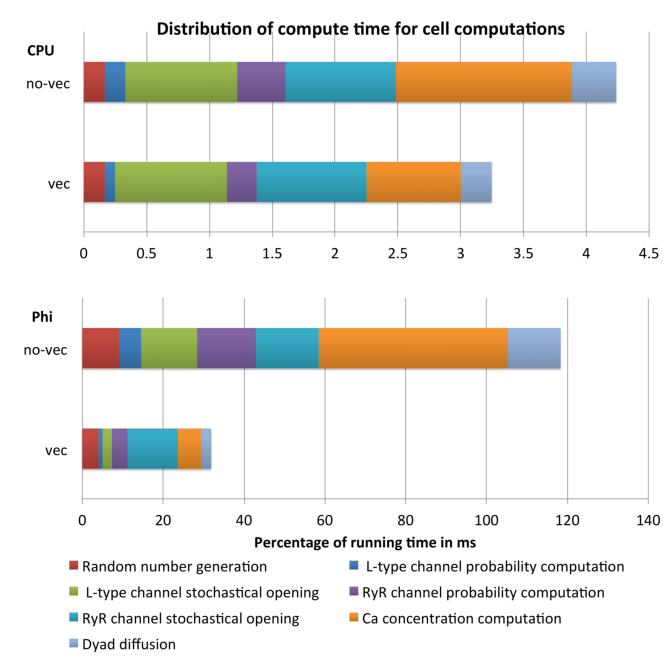
\includegraphics[width=\linewidth]{figs/perf1crop.pdf}
%\end{center}
\caption{Performance improvement of the individual functions in the dyad computations due vectorization. For the Xeon Phi, this also includes the conservation of random numbers.
Note the change in scale due to the low single-core performance of the Xeon Phi. Performance is reported per time step, based on a measurement over 10,000 time steps.}
\label{fig:optimizations}
\end{figure}

第二个实验是检验单个Xeon Phi设备上的扩展性,包括弱扩展和强扩展。由于存储的限制,弱扩展实验中让每个线程处理8个细胞,则224个线程最多处理$8\times224$个细胞,基本达到单个Xeon Phi设备的存储上限。在强扩展试验中,单个设备的处理的细胞数也为$8\times224$,考虑到执行时间长短的因素,强扩展试验至少使用的线程数为$16$。图\ref{fig:scaling}是强扩展和弱扩展试验中的使用不同线程数下模拟10000个时间步的执行时间,如果将执行时间转化为每秒钟细胞计算数这个指标,这个指标在强扩展和弱扩展中基本相同,所以强扩展和弱扩展的性能差别不大。从试验结果还可以发现,当使用到56个物理线程时,可以观察到非常好的扩展性,能达到$86\%$的效率。而在使用线程数超过56时,扩展性有所下降,这是由于小核的存储带宽竞争变激烈导致的。当使用到112个线程时,效率下降到$65\%$了。当线程数目超过了物理核数时,除了存储带宽方面的竞争,如果两个线程共享一个物理核,则每个线程的cache大小将减少,这也将影响性能的发挥。当设备中创建224个线程时,两个线程共享时钟周期,虽然没有使用更多的硬件资源,但可以观察到明显的性能提升。从线程使用的角度看,虽然效率下降了,但相对于资源使用的角度看,其实效率是相当高的。这些现象和数据表明,模拟性能很大程度上受限于延迟而不是吞吐量,因此超线程的使用能缓解这个问题。

\begin{figure}[htb]
%\begin{center}
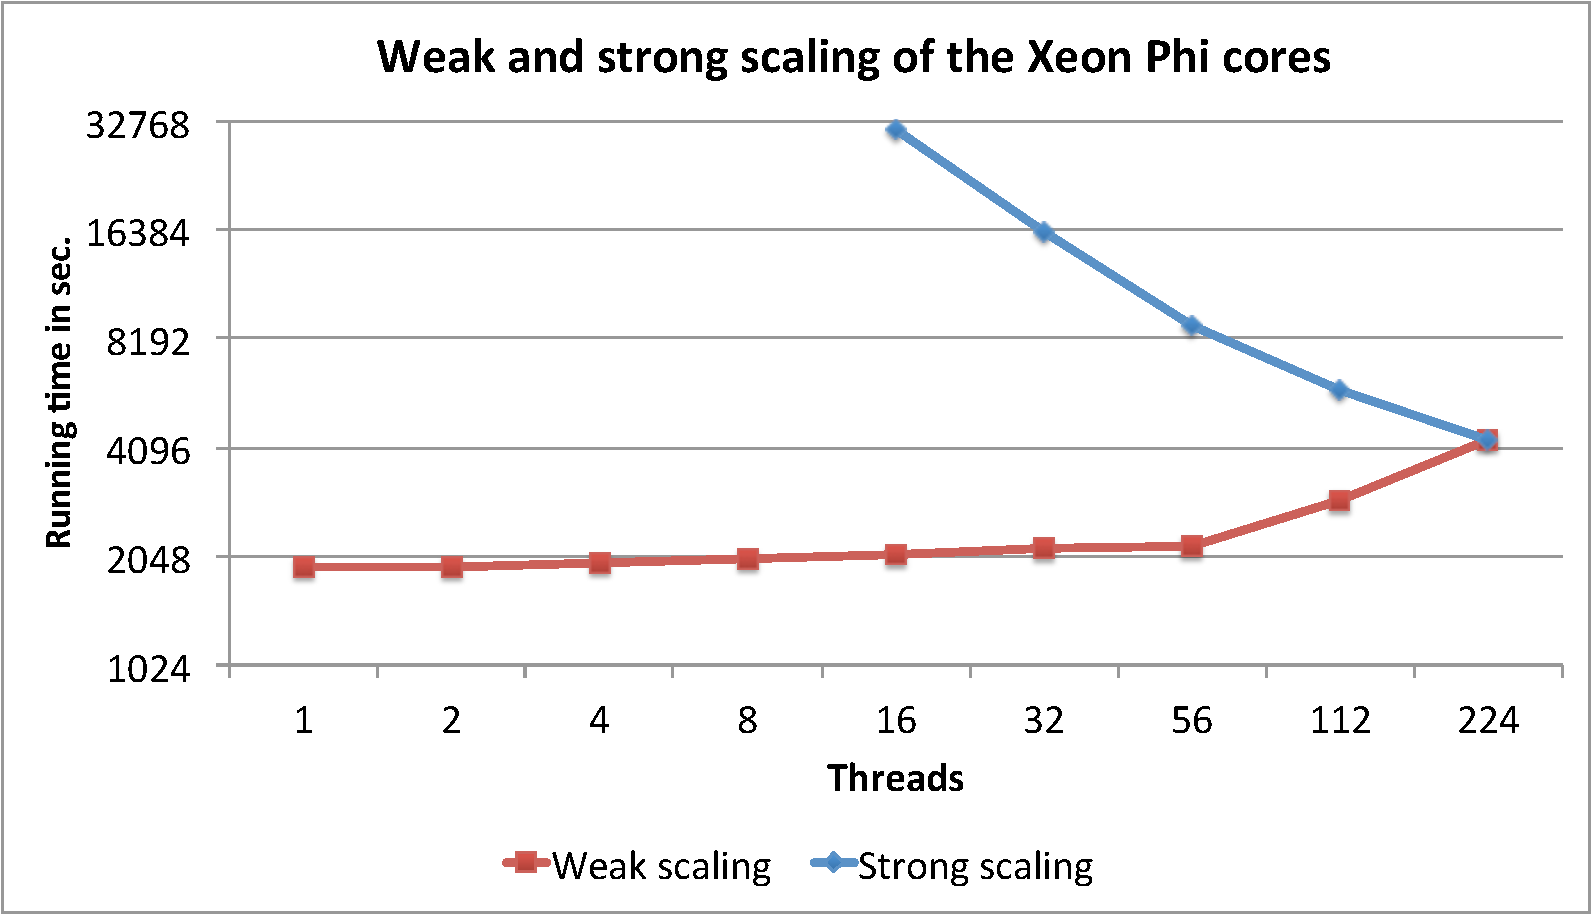
\includegraphics[width=\linewidth]{figs/weakstrongscalePHI.pdf}
%\end{center}
\caption{Weak and strong scaling on a single Xeon Phi, shown as running time over 10,000 time steps for $8$ cells per thread in weak and 1,792 cells in strong scaling.}
\label{fig:scaling}
\end{figure}

在Ivy Bridge CPU上做了同样的强扩展和弱扩展试验,唯一不同的是模拟的规模,弱扩展试验中,每个小核负责8个细胞的计算,强扩展中需要完成$8\times24$个细胞的计算。在Ivy Bridge CPU上取得与Xeon Phi上相似的扩展性,除了Ivy Bridge CPU不支持超线程试验,因此被使用的物理核的数目与创建的线程数时钟保持一致。详细的试验结果可以参考图\ref{fig:scaling2}。扩展性因为存储带宽达到饱和而受限,即当每个socket中使用的物理核数超过两个时,性能没有与使用的物理小核数保持线性增长。

\begin{figure}[htb]
%\begin{center}
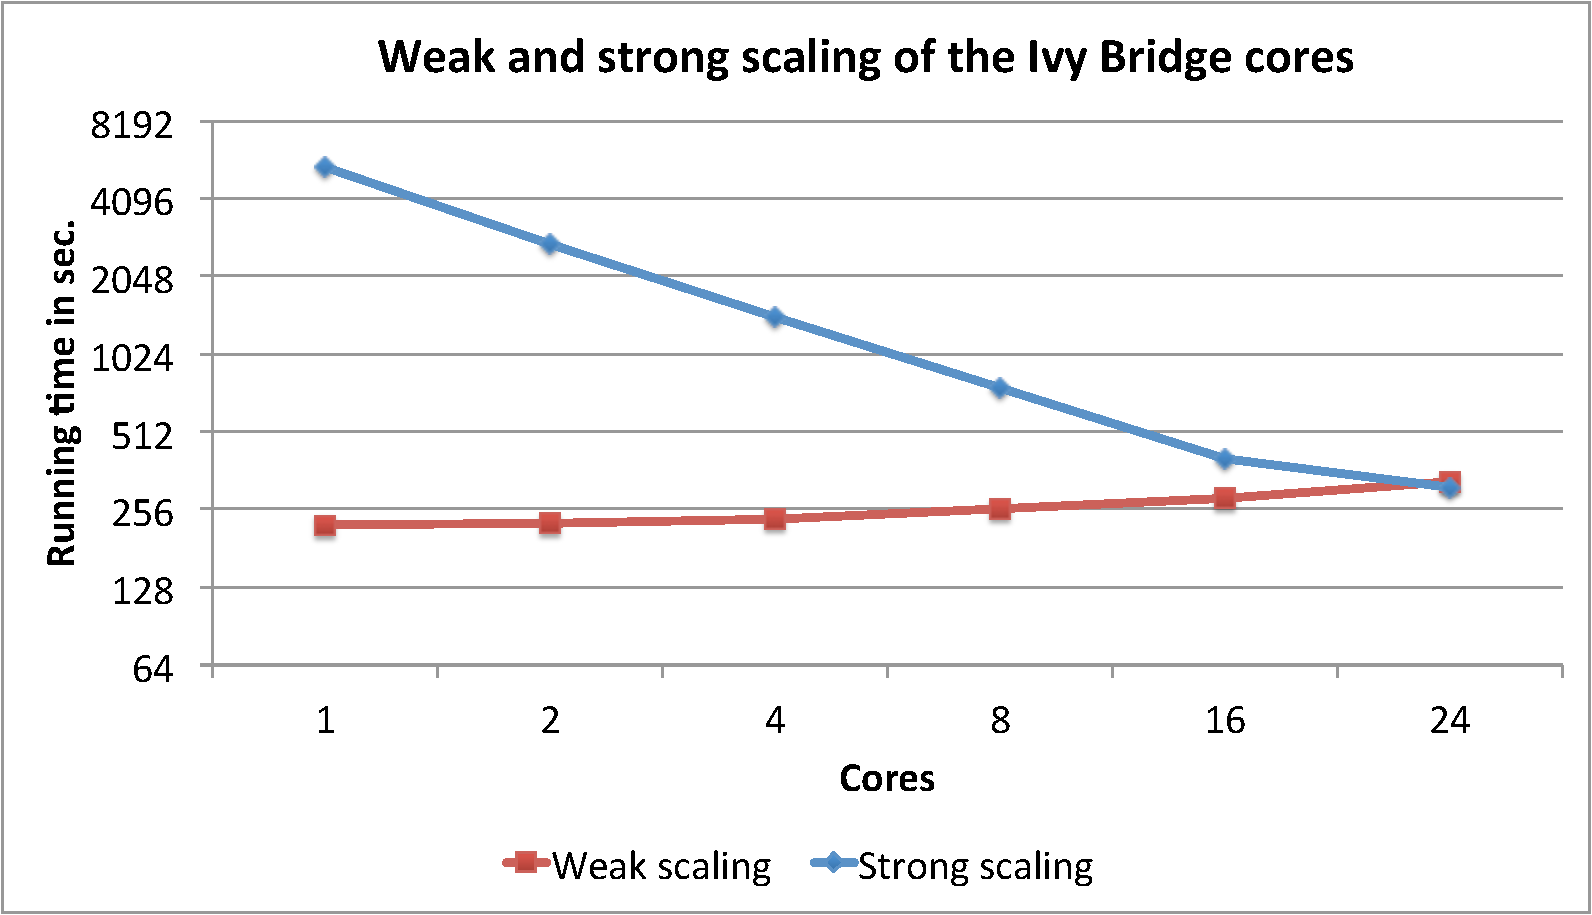
\includegraphics[width=\linewidth]{figs/weakstrongscaleCPU.pdf}
%\end{center}
\caption{Weak and strong scaling on the CPU, shown as running time over 10,000 time steps for $8$ cells per thread in weak and 192 cells in strong scaling. Threads are distributed evenly over both sockets.}
\label{fig:scaling2}
\end{figure}

\subsection{心脏组织模拟的单节点性能}
第三个实验测试了单个节点在心脏组织模拟计算中的性能。节点的每个Xeon Phi设备被分配$8\times224$细胞,Xeon CPU上分配$2624$个细胞,共$20\times20\times20$个细胞,这些细胞构成一个三维的网格。表\ref{tbl:perf1}是试验结果,注意到,每次都是分配细胞给节点上的两个CPU主机,因此测试的是2个CPU的性能。显然,单节点内的Phi的性能是相对稳定的。然而,由于技术原因,节点内的各个Phi的时钟周期会有所差异,因此,在某些节点上负载均衡问题会比预期的差些,导致CPUs处于等待状态。

\begin{table}
\caption{Single and aggregate performance of the devices within a node. CC/s is the number of cell computations per second.}
\label{tbl:perf1}
\begin{center}
\begin{tabular}{c|ccc}
Device & Cells & Time (in sec.) & CC/s \\
\hline
2 CPUs	&	2,624	&	1,706	&	6,152	\\	
1 PHI	&	1,792	&	1,859	&	3,856	\\	
2 PHIs	&	3,584	&	1,860	&	7,708	\\	
3 PHIs	&	5,376	&	1,861	&	11,555	\\	
2 CPUs+3 PHIs	&	8,000	&	1,879	&	17,030	\\	
\end{tabular}
\end{center}
\end{table}

图\ref{loadbalance}表示的是负载均衡的情况。虽然节点内的通信占用了不是特别重要的时间,但不完美的负载均衡可以导致CPU等待约$10\%$的计算时间。可以看出异构计算对负载均衡问题是非常敏感的,实际上,如果CPU展示的性能比预期的还差,则因为Phi而导致等待的时间将变得更大。由于单个节点每次处理的细胞都是立方体的限制,一个完美的负载均衡是不可能达到的。

\begin{figure}
 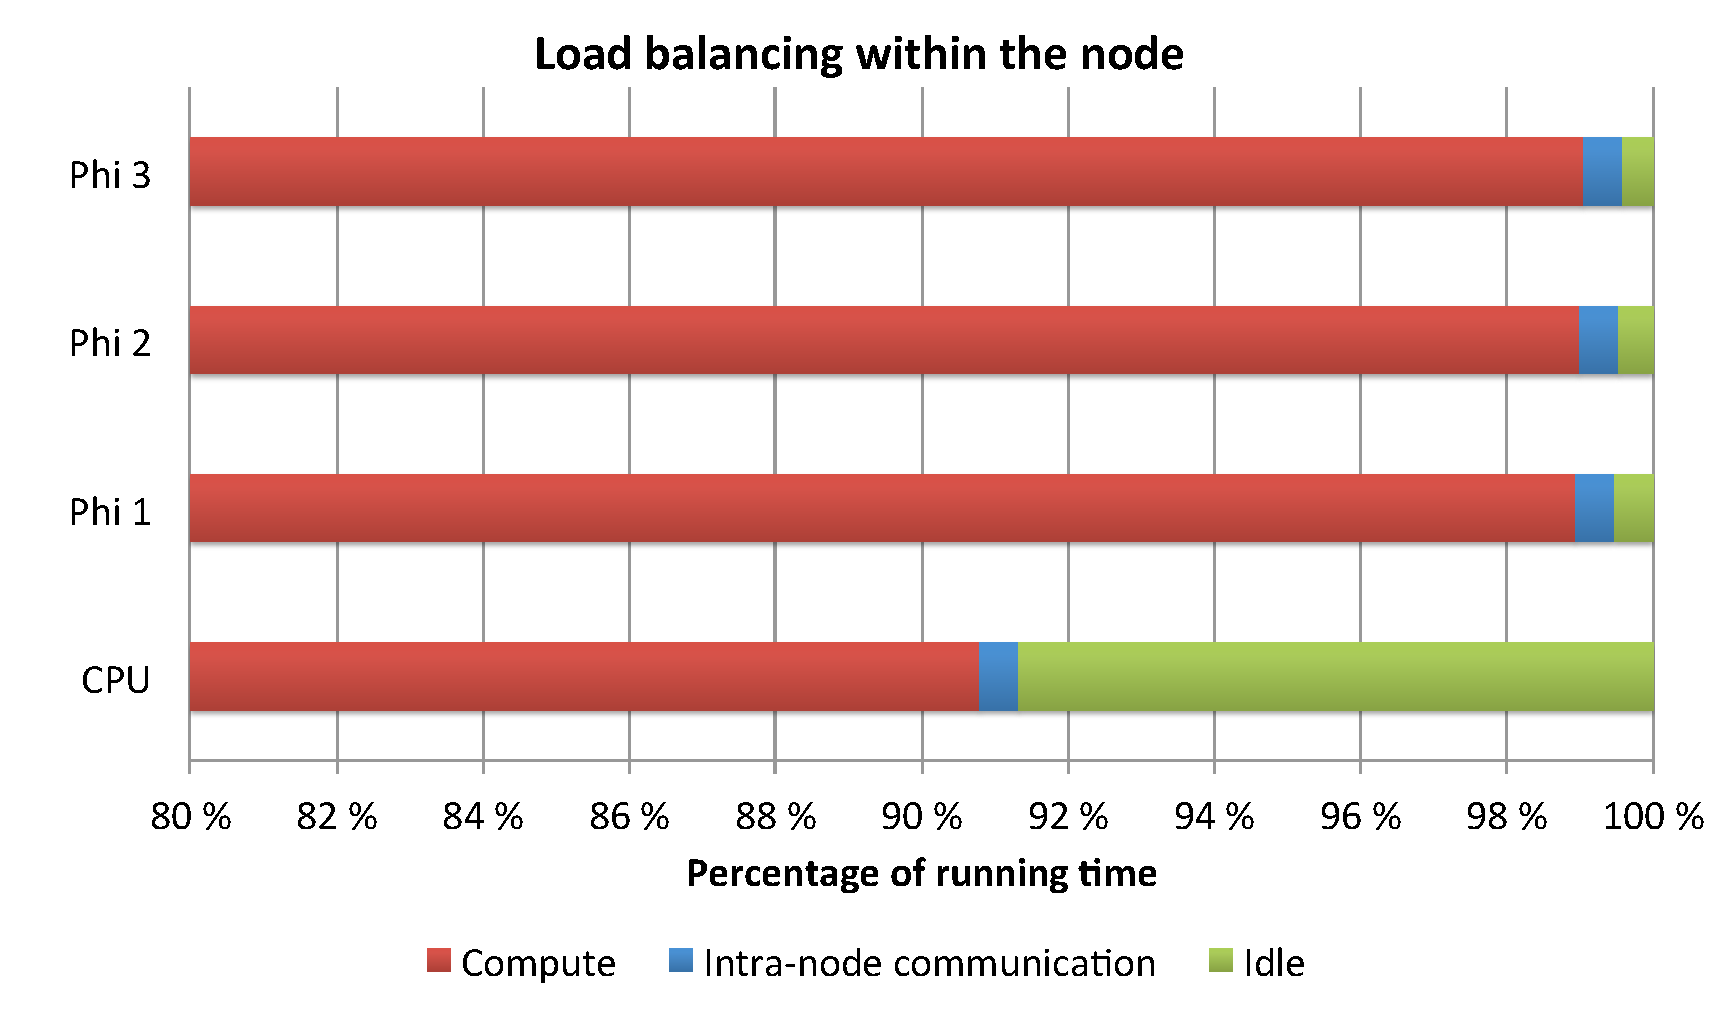
\includegraphics[width=\linewidth]{figs/loadbalance.pdf}
  \caption{Load balancing within the node. The communication overhead is insignificant, but the imperfect load balancing is noticeable. (Percentages which are not show consist of compute time for all devices.)}
  \label{loadbalance}
\end{figure}

\subsection{心脏组织模拟在多节点上的扩展性试验}
基于单节点的性能,本课题进一步对大规模多节点上的性能也进行了测试评估,包括节点间的通信以及扩展性两方面。图\ref{weak_scale}展示的是从1到512个节点的弱扩展性结果,由于MPI通信开销小,取得了几乎完美的扩展性。另外,在本次试验中,节点间的负载均衡问题对性能影响非常小。

每个试验中采用的子域规模为$20\times20\times20$,这些细胞构成一个立方体形状。则400个节点可以处理的心脏组织规模可以达到$400\times400\times20$,通信开销只占总时间的约$1.76\%$,需要说明的是,由于Phi节点使用数目的限制,通信测试基于的计算都是在CPU上的计算。但这对研究通信开销是没影响的,因为异构节点间的通信也是由CPU完成的。如果通信按照这种趋势发展的话,可以预测使用天河2号上所有的16000个节点计算的话,通信所占的比例也不会超过$6\%$,因此心脏组织模拟应用能够很好地扩展到更大规模的节点中运行。

\begin{figure}
 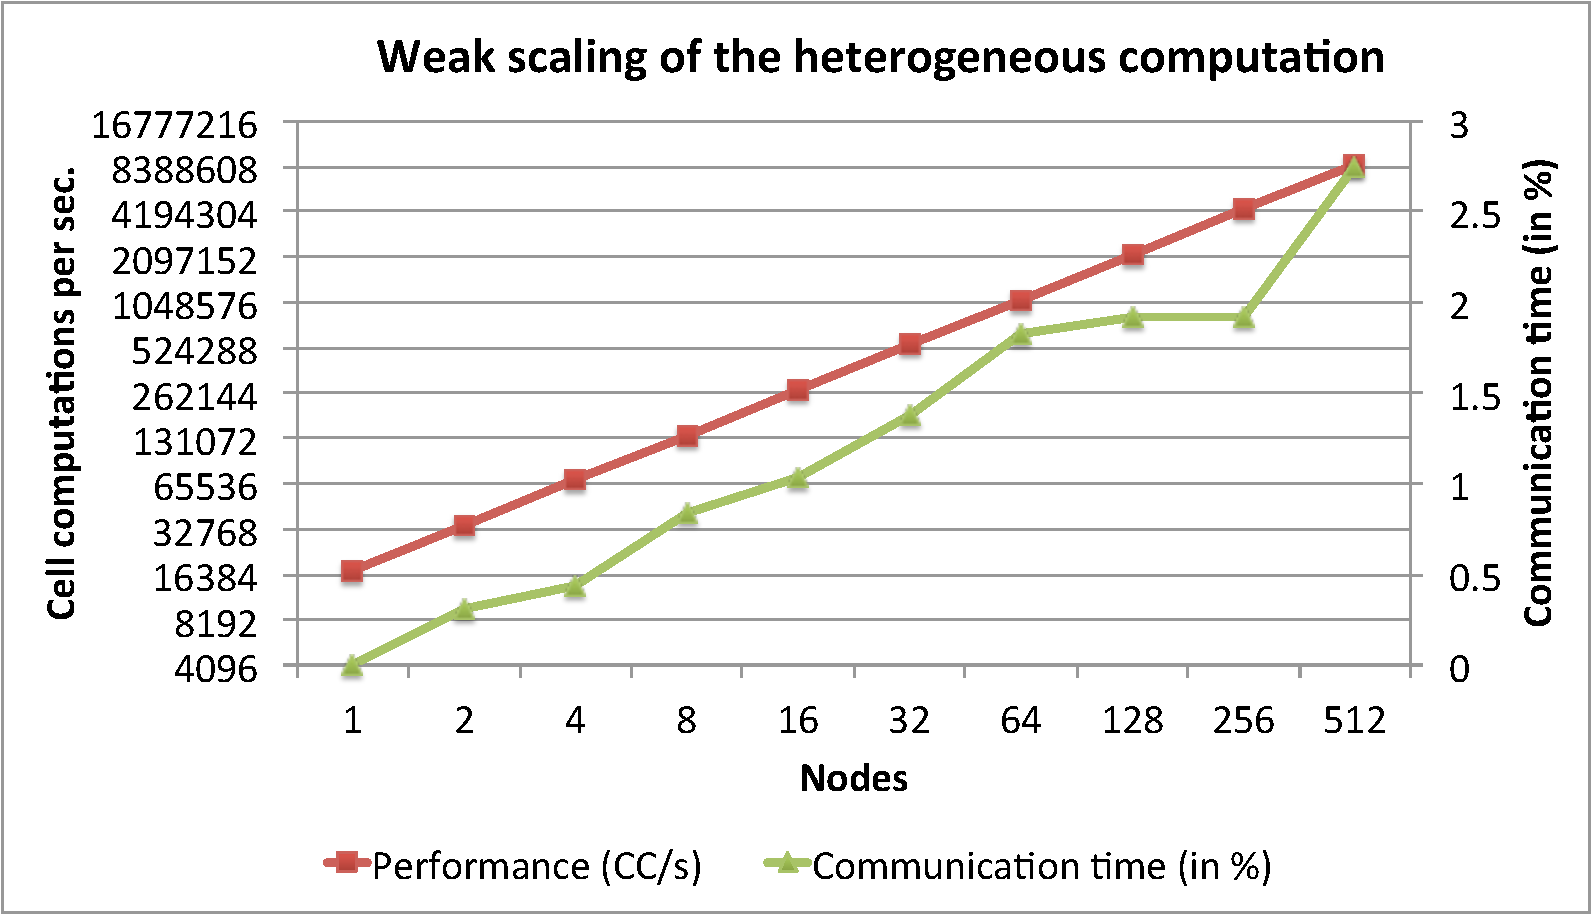
\includegraphics[width=\linewidth]{figs/weakscaling.pdf}
  \caption{Weak scaling of the overall simulation. The communication overhead remains below $3\%$, allowing for near perfect scaling.}
  \label{weak_scale}
\end{figure}

\subsection{心脏组织模拟试验}
本节试验中,展示了在正常情况下的心脏组织细胞模拟结果。

在心脏心室中截取大小为2 mm$\times$32 mm$\times$32 mm的组织进行正常的活化试验,结果如图\ref{fig:activation}所示。试验中,组织的某个面的所有细胞在t = 0 ms受到一个人为的刺激,这种刺激主要是将这些的细胞的电压变高,模拟的过程中,可以看到电压将沿着直线向某个方向传播,整个组织的细胞经过约70 ms都被极化。因此,可以估算出传导的速度大约为45.7 cm/s,这个速度与文献\upcite{durrer1970total}中报告的速度46.4 cm/s是接近的。

\begin{figure}
 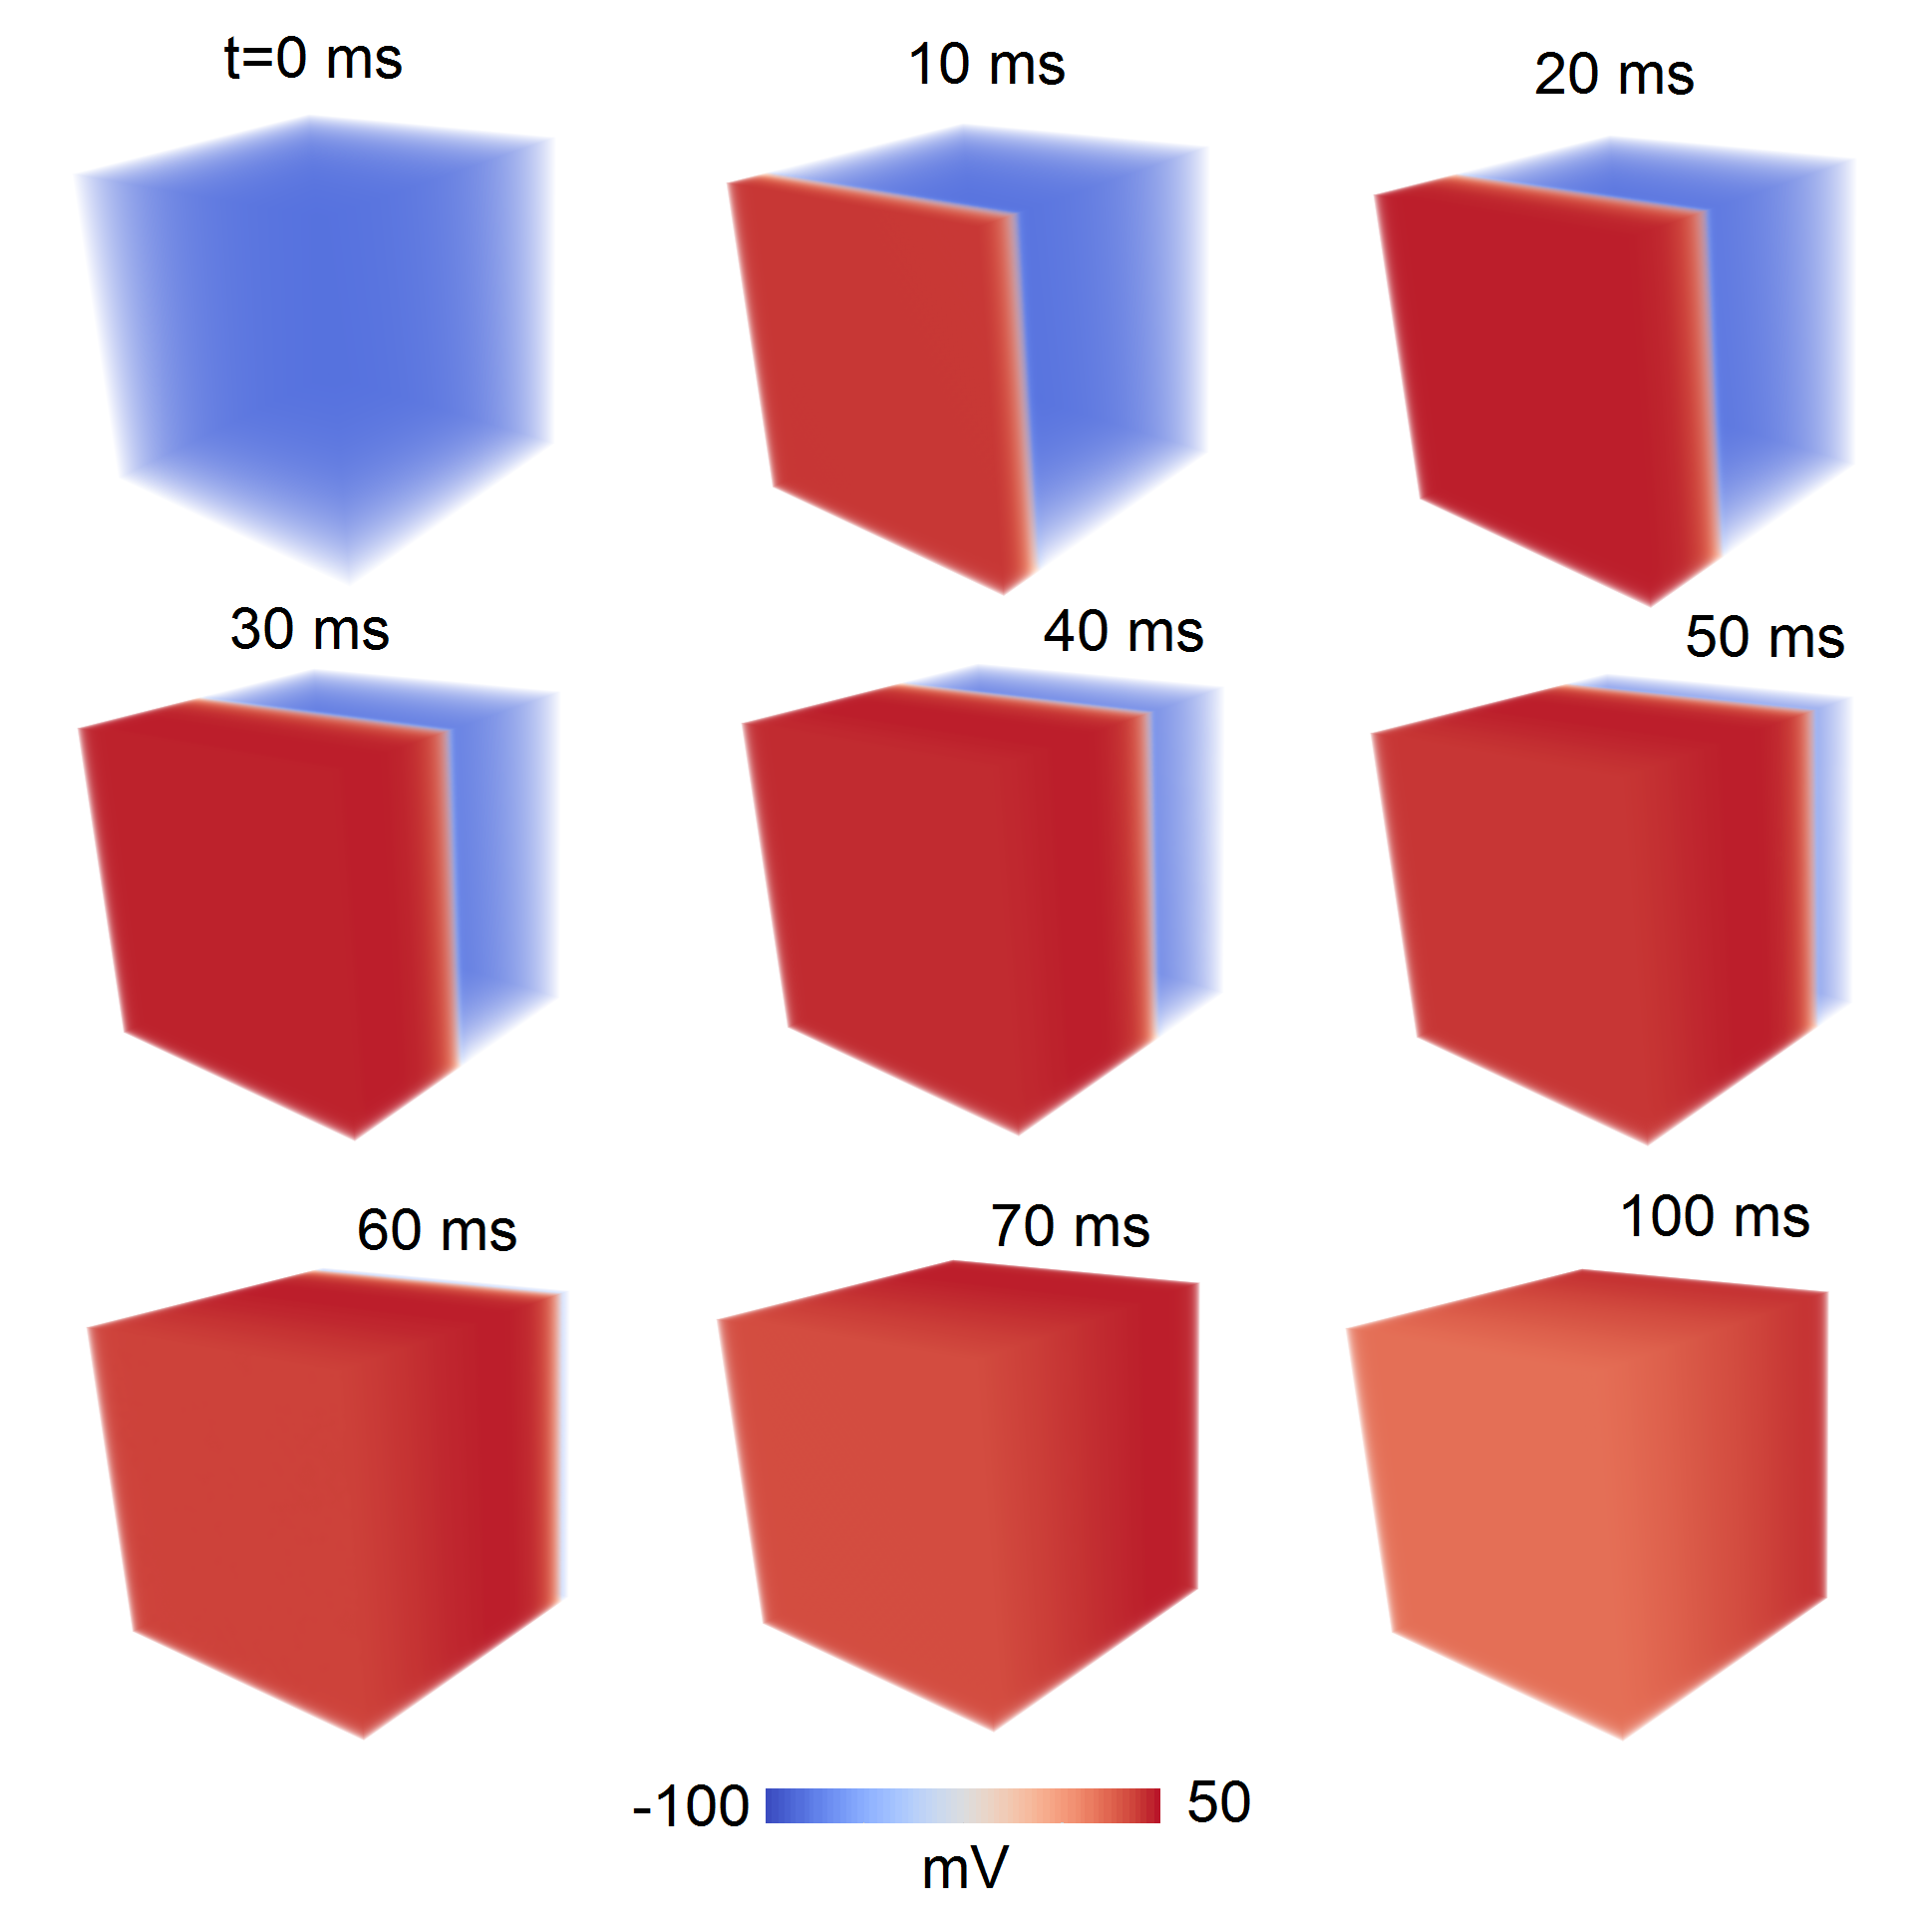
\includegraphics[width=\linewidth]{figs/tissue_activation.png}
 \caption{Activation pattern in a 3D human ventricular tissue.}
 \label{fig:activation}
\end{figure}

\begin{figure}
 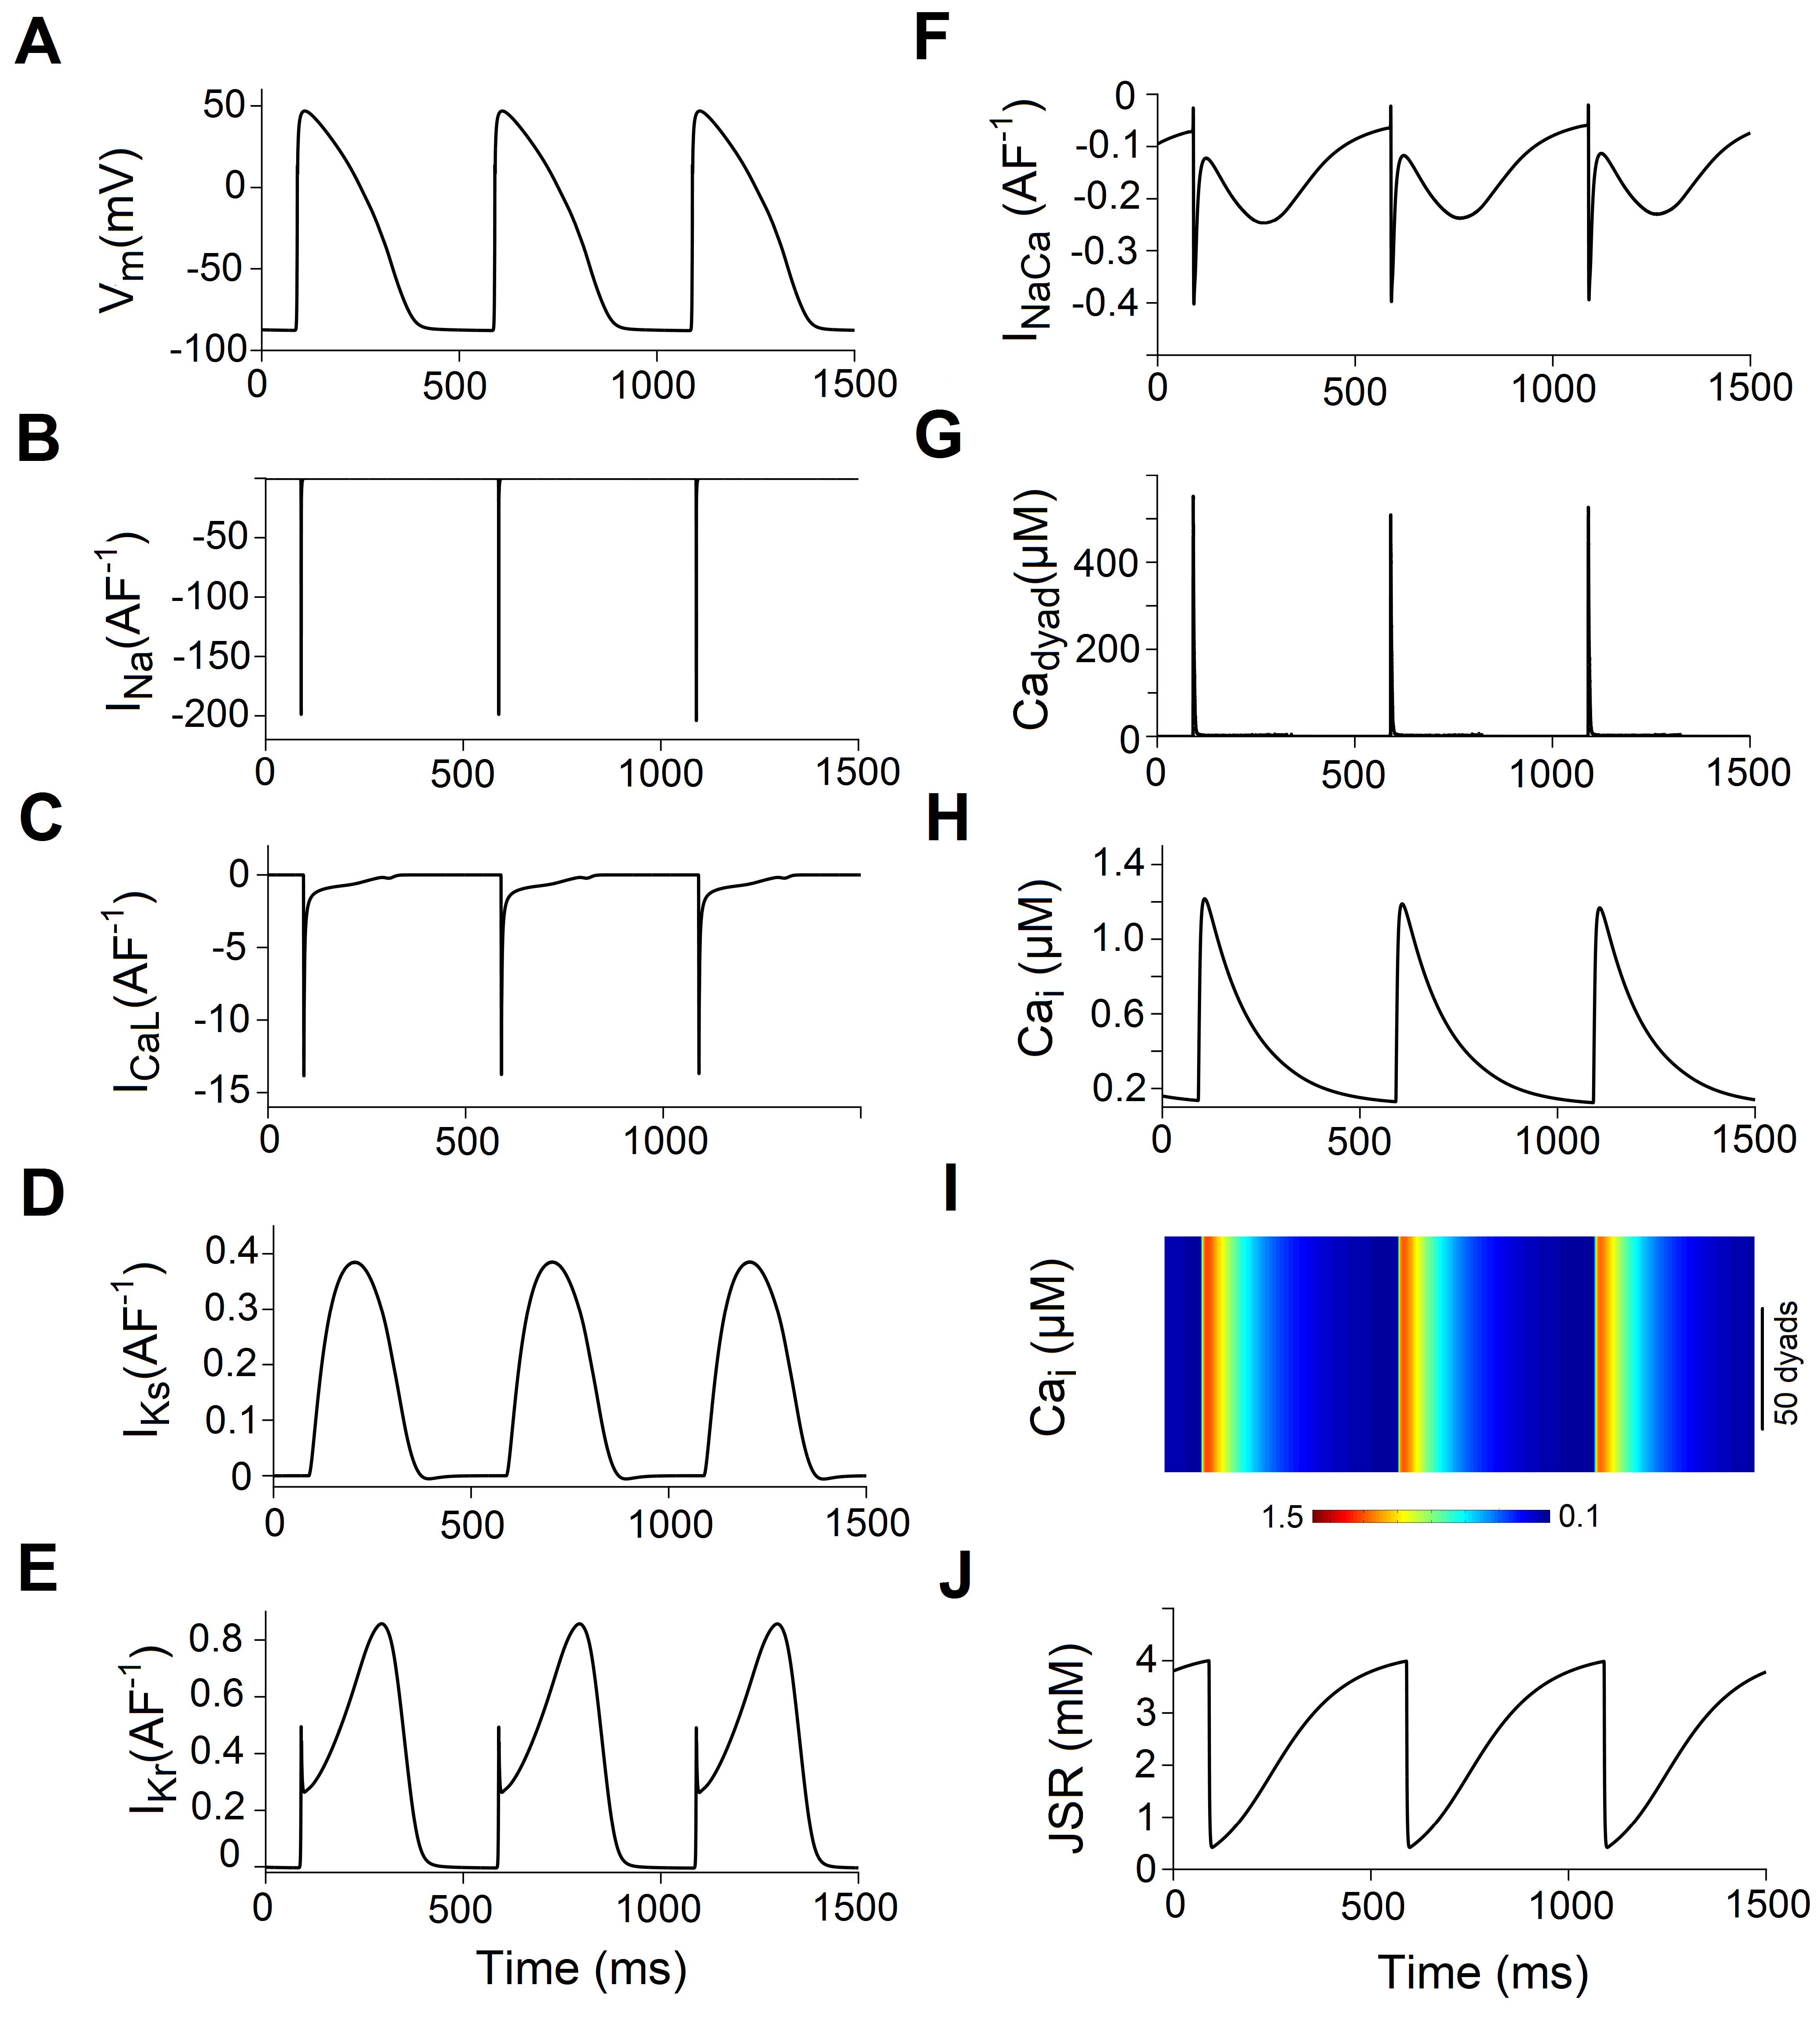
\includegraphics[width=\linewidth]{figs/cell_variables.png}
 \caption{Action potentials (AP), electrophysiological currents and calcium concentration (Ca) values in a 3D tissue-center cell at steady-state. (A) Membrane voltage ($V_m$) (B) Fast Na current ($I_{Na}$) (C) L-type Ca current ($I_{CaL}$) (D) Slow component of delayed rectifier K current ($I_{Ks}$) (E) Rapid component of delayed rectifier K current ($I_{Kr}$) (F) Na-Ca exchange current ($I_{NaCa}$) (G) Ca in the dyadic space ($Ca_{dyad}$) (H) Intracellular Ca in the myoplasm ($Ca_i$) averaged over 10000 dyads (I) Simulated line-scan image of $Ca_i$ along the long-axis of the myocyte and (J) Junctional sarcoplasmic reticulum concentration (JSR) averaged over 10000 dyads.}
 \label{fig:calcium}
\end{figure}

心脏组织模拟过程中,处在组织中央的细胞的动作电势、重要的电生理电流以及钙离子浓度变化如图\ref{fig:calcium}所示,模拟持续3个正常的心跳周期,每个周期为500 ms。图\ref{fig:calcium}的A部分是活动电势变化,而B、C、D、E以及F中显示的是各种离子电流变化,H和J是所有dyad的钙离子平均浓度变化,这些结果与ORd模型\upcite{o2011simulation}中的结果是一致的。相关的细胞内钙离子在肌质($Ca_i$)沿着肌细胞中轴线以及钙离子在dyadic空间($Ca_{dyad}$)的线扫描图分别为图\ref{fig:calcium}中I和G所示。这些结果证明了本课题开发的3D组织模拟器在模拟正常的心脏活动中的相关结果与现有已经发表的结论是一致的。

\section{小结}
在心脏组织层级以及器官级的异常活动研究在计算医学领域仍然是一个突出的课题。采用精细的细胞模型进行大规模的模拟能够帮助心脏病专家理解细胞内钙离子处理异常对心律失常机制的理解。

本课题在天河2号这样的高性能计算系统上实现了心脏组织的模拟,支持大规模节点的模拟。虽然在节点内Xeon Phi上高度优化的代码的性能比节点中的2个Ivy Bridge CPU的性能低些,并且比Xeon Phi的峰值性能也低很多,但已经取得的性能与其它很多研究\upcite{CMPST13,VGGR14}所取得的性能接近,其它研究也说明了在开发Xeon Phi的潜在性能上的挑战与困难。并且Phi加速设备上能够提供的最大全局存储大小成为模拟规模的最主要限制。虽然理论上可以在CPU主机与Phi加速设备间交换数据,CPU上主存大小为$64$~GB,意味着Phi设备上模拟的规模最多只能扩大一倍,因为每个Phi设备原本全局存储为8GB,再加上对应CPU上需要12GB大小的存储,这就需要消耗CPU36GB的存储了。

然而,未来的超级计算机系统比如NERSC Cori以及其它在CORAL\upcite{coral}的机器将使用新一代Xeon Phi体系结构(KNL),新一代的Xeon Phi加速器将拥有更大容量的全局存储。Cori系统的每个设备将具有$96+16$~GB的存储。虽然9300个这样的节点还不足于模拟整个心脏,但是,即将建好的Aurora超级计算机具有50000个节点,对于整个心脏的模拟是足够的。因此,我们的模拟器将在不久的将来可以对心脏器官进行模拟。

在大量的优化工作中,除了算法上的改进,比如采用二项分布采样以及节约随机数的使用,对性能提升最大的是手动和自动向量化技术的使用。并且,对OpenMP并行化的正确使用对于在众核系统上获得高性能发挥着重要作用。对于Xeon Phi的代码的优化技术同样适应其它科学计算应用的代码,另外,本章的试验结果表明由于代码的复杂性,该应用属于延迟受限的应用,因此,超线程技术在不需要任何额外代价就能提高额外的性能。这对一般的简单计算kernel是不适应的。

对于异构计算来说,本课题选择了一种层次化的领域分解方法,每个计算节点被分配一个子域任务的计算,分配到每个节点的子域又进一步在计算设备间切分。从编程的角度来看,除了在负载均衡方面能获得灵活性的好处,这种任务划分方式使得节点间通信和节点内的计算很好的分开,使得代码在其它超级计算机系统中具有很好的移植性。

本课题在未来的工作中,还会继续尝试在其它加速设备上,比如GPU上,或者新一代的Xeon Phi加速器上进一步优化。